\section{\ecb pinch observations}\label{sec:eb_pinch}

As mentioned in the previous section, the ionization rates in the core are insufficient to account for the electron density increase observed. Additionally, the impurity contribution to the electron density rise is small in order of magnitude compared with what is 'needed'. This presents a dilemma for the model since quasi-neutrality dictates that the ion density rise with that of electron, but if a source for this 'extra' density is to be assumed, then the temperature of this ion source is also to be assumed. From a ion thermal modeling point of view, allowing an arbitrary temperature to be associated with an anomalous density term is problematic as it can be a large thermal term compared to the other mechanisms, and allowing it to be adjusted at will on the researcher's (my) whim weakens the validity of the model. It would be much preferable for the mechanism to be discovered instead being assumed. 

\begin{figure}
    \centering
    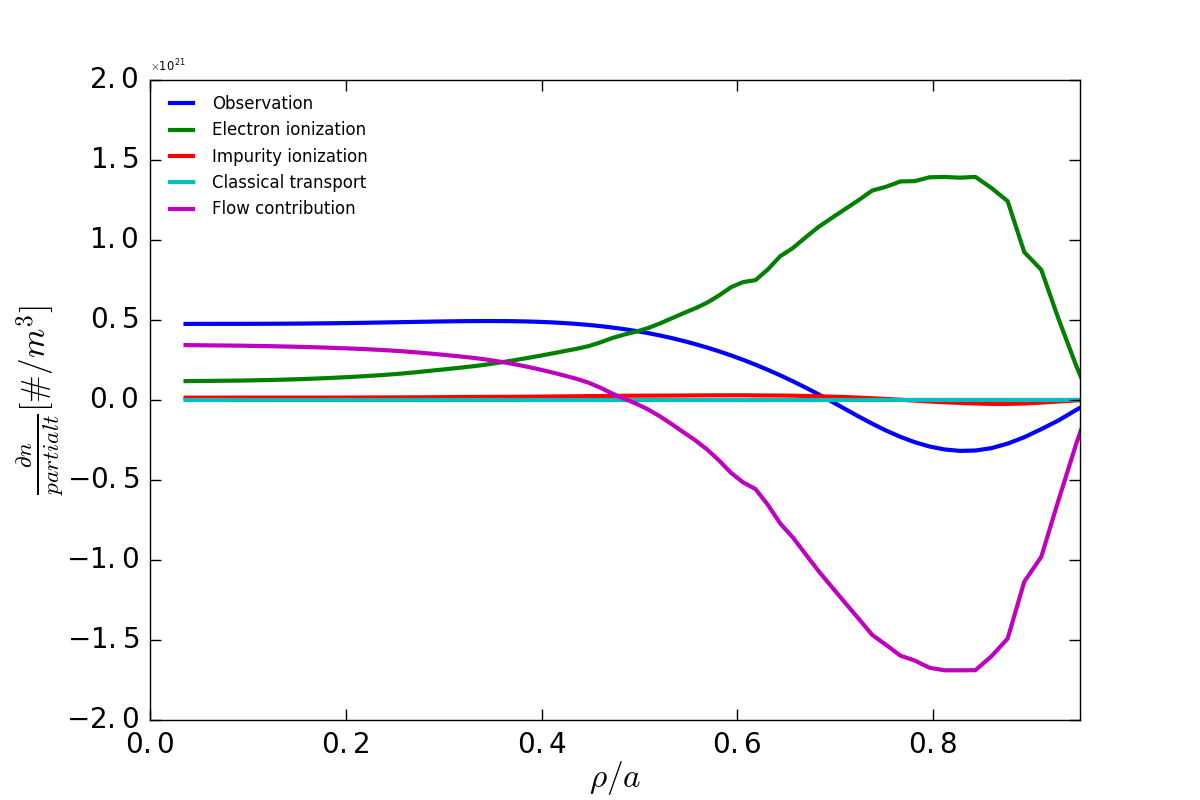
\includegraphics{ion_transport_results/density_balance.png}
    \caption[$\partialt n_e$ in MST and their sources]{$\partialt n_e$ in MST and their sources. This particular plot presents the ensembled analysis at 14ms.}
    \label{fig:density_balance}
    %%TODO, need larger legend text.
\end{figure}

The first step is realizing that source rate mechanisms are limited. Ionization of deuterium and impurities accounts for all the available sources of electrons. However, particle flow has not been explored to the same degree. In J. Reynolds's thesis on simulating the effect of PPCD using the numerical MHD code NIMROD \cite{Reynolds2007}, he observes the simulation undergoing an inward pinch flow across the simulated plasma volume (see figure \ref{fig:NIMROD_pinch}). He also refers to previous simulation studies on PPCD-like conditions showing inward pinch\cite{Puiatti2003, Ashida2005, Svidzinski2007}. More empirical on MST, PPCD drive the plasma into deep reversal and the reversal surface moves inwards during this process. Previous measurements of electron density using FIR also show the gradient region moving inwards (figure \ref{fig:ne_gradient_pinch}), hinting at a pinch. After all, it is in the name of the configuration.

\begin{figure}
    \centering
    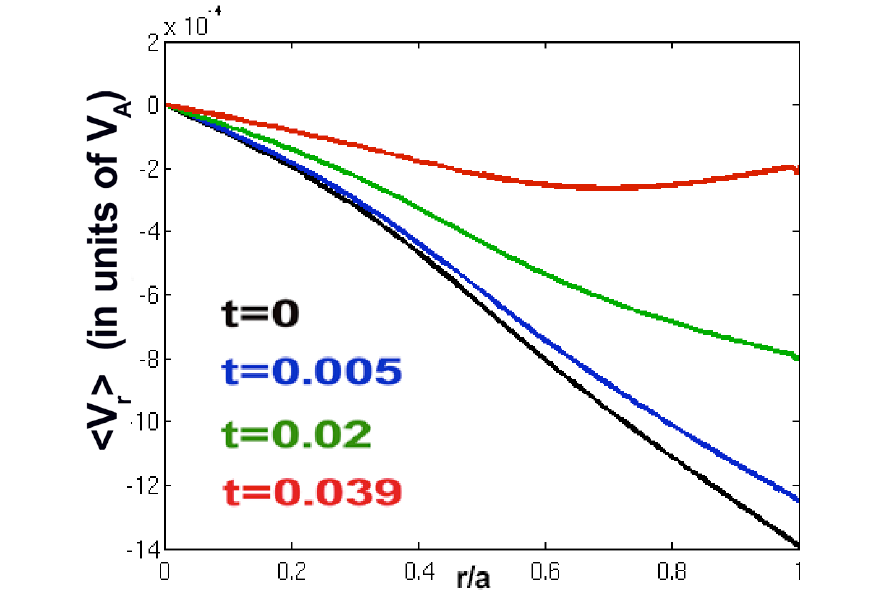
\includegraphics[width = 5.5in]{ion_transport_results/reynold_pinch.png}
    \caption[Pinch velocity from J. Reynolds' simulations]{Pinch velocity from J. Reynolds' simulations. Note that the simulation volume ends at the reversal surface and the Lunquist number of the simulation is lower than actual plasma conditions. (Reproduced from J. Reynolds\cite{Reynolds2007}). }
    \label{fig:NIMROD_pinch}
\end{figure}

\begin{figure}
    \centering
    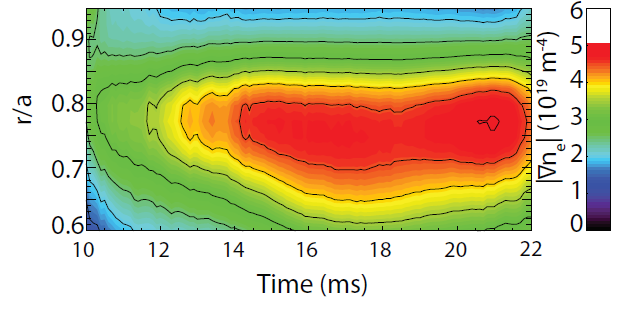
\includegraphics[width = 0.8\linewidth]{ion_transport_results/duff_gradient.png}
    \caption[Evolution of the $n_e$ gradient during PPCD]{Evolution of the $n_e$ gradient during PPCD. (Reproduced from J. Duff \cite{Duff2018})}
    \label{fig:ne_gradient_pinch}
\end{figure}


Working with the hypothesis that the unaccounted for core density rise is due to a pinch flow, I use the continuity equation (equation \ref{eqn:continuity}) to calculate the particle flux needed to balance out the observations. This forms a basis for comparison with the hypothesized mechanism, \ecb drift.

%\subsection{Estimating radial \ecb drift}

MST have limited ability to diagnose $\vec{E}$ field in high current plasmas. Thus the $\vec{E}$ needs to be estimated from indirectly from the $\partialt\vec{B}$ according to the Maxwell equations. The $\vec{B}$ field are calculated by the equilibrium reconstruction code MSTfit using inputs from the gap voltage measurements, edge pick up coils, and FIR polarimeter measurements. Sequential MSTfit equilibrium reconstruction are used to estimated $\partialt\vec{B}$. From there $E_{pol}$ can be calculated through:
\begin{align}
   E_{pol}(\rho_v) & = -\frac{1}{\rho_v}\int_{0}^{\rho_v}\rho_v' \frac{dB_{tor}}{dt} d\rho_v'
\end{align}
where it is taken as a boundary condition that the $E_{pol}$ is zero at the magnetic axis.

The calculation of $E_{tor}$ is slightly more complicated, as it is a function of major radius and not $\rho_v$. The voltage measurement ($V_{PG}$) across the poloidal gap on MST (a cut in the vacuum vessel along its intersection with the poloidal plane) is a reflection of the toriodal E field at the wall and serves as the boundary condition for the integration. $E_{tor}(R, Z=0)$ along the Z = 0 plane is determined as a function of major radius (R) through:
\begin{align}
\oint_S \vec{E}\cdot d\vec{l} &= -\iint \frac{\partial}{\partial t}\vec{B}\cdot d\vec{s}\\
E_{tor}(R) 2\pi R &= -\int_0^{2\pi}\int_{R_{in}}^{R}R'\frac{\partial B_{pol}}{\partial t} d\phi'dR' - V_{PG}\\
E_{tor}(R) &= -\frac{1}{R}\int_{R_{in}}^{R}R'\frac{\partial B_{pol}}{\partial t} dR' - \frac{V_{PG}}{2\pi R}\label{eqn:E_tor}
\end{align}
where $R$ refers to the major radius, and $R_{in}$ is the major radius at the inboard wall. To incorporate into the 1-D approximation, the inboard and outboard $E_{tor}$ is averaged according to their flux surface subsequently. From these, we can calculate the radial \ecb flux,
\begin{align}
    \Gamma_{\vec{E} \times \vec{B}} &= n_e v_{\mecb} \nonumber \\
    &= n_{e} \frac{E_{pol}B_{tor} - E_{tor}B_{pol}}{B^2}
\end{align}
The result of this calculation is shown in figure \ref{fig:eb_flux}. This is compared with the observed flux calculated from the continuity equation. The result show that \ecb is a good explanation for the inwards flow needed to balance out the observations in the core. Hence, the $\partialt n_e$ rise in the core can now be accounted for in such a way that the associated ion temperature is no longer arbitrary, since \ecb flow is ambipolar.

%\begin{figure}
%    \centering
%    \includegraphics{ion_transport_results/eb_v.png}
%    \caption[Calculated \ecb pinch velocity]{Calculated \ecb pinch velocity. The velocity is plotted to the reversal surface. Compares well with MHD simulations results in figure \ref{fig:NIMROD_pinch} qualitatively. }
%    \label{fig:eb_v}
%\end{figure}
\begin{figure}
    \centering
    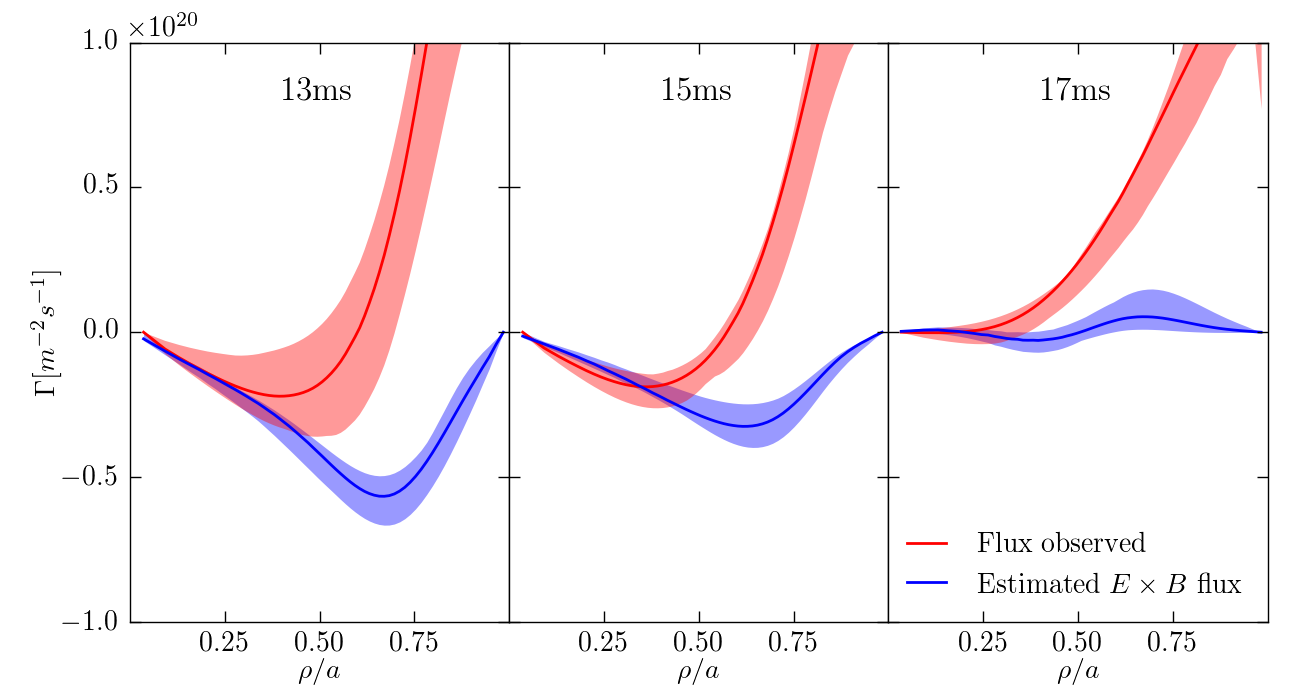
\includegraphics[width=\linewidth]{ion_transport_results/flux_comp.png}
    \caption[\ecb flux compared to measured flux]{\ecb flux compared to the observed flux. 'Observed' flux is that implied by the continuity equation though $\partialt n$ and source rate observations. The plot is somewhat zoomed in to show the dynamics in the core, where the previously discussed 'need' for an inward flux to account for the observations are. The outer areas of the plasma is dominated by an outward anomalous particle flux. The outward flux at the edge is consistent with previous measurements.\cite{Lanier2001a}. }
    \label{fig:eb_flux}
\end{figure}
%section{Flow effect on heating}
The effects of the flow can be calculated via the method laid out in section \ref{sec:flow_effects}. It is useful reiterate the two components of the flow effect. One has to do with the conservation of the energy being carried by the ions. This term brings energy into the core, but generally will result in cooling, whereas it brings energy out of the edge (loss to wall), but is general increasing temperature as they are 'replaced' by ions flowing out from mid-radius. The other term is the compressional work by the \ecb drift in varying fields. This is calculated from the estimated drift velocity, and is a mostly positive term, and since it doesn't not have density effects, it represents a temperature increase. The calculations show that the compression is a nearly global heating term that goes away during the PPCD period (refer to figure \ref{fig:power_terms_with_adhoc}, where as the flow conservation term is a large energy loss term outside of mid-radius, but brings some energy to the core with the ions when compression is active. It should be noted that the flow conservation's term's effect on temperature is nearly the opposite, as during compression, it brings cool ions into the core, and in the edge, it brings hotter ions out increasing the local temperature (refer to figure \ref{fig:temperature_change_zoomed}).